\chapter{\kl{CN} Comparison and Feedback}

\margintoc{}

In this chapter, I will discuss the reality and expectations of how usable a
verification tool for C \emph{can} be at this stage. I will start with my brief
and informal comparison between \kl{CN} and similar tools, based on my
experience of verifying \kl{pKVM}'s simpler
\href{https://github.com/rems-project/CN-pKVM-early-allocator-case-study}{\emph{early}
allocator}, in \kl{CN}, \kl{VeriFast}~\cite{jacobs2011verifast} and
\kl{Frama-C}~\cite{baudin2021dogged}. I will also discuss a
\kl{RefinedC} verification of the same, which was completed by the
developers~\cite{sammler2021refinedc}. Part of this comparison was featured
in~\textcite{pulte2023cn}, including the annotation overhead and execution
times.

After that, I will discuss some feedback given by some industry partners on
\kl{CN}. As an academic, these seem borderline unreasonable, especially when
compared to the aforementioned state-of-the-art research tools, but as an
ex-industry professional, it is much easier to concede. Given our goal of
targeting kernel programmers, we as academics want industry adoption for these
tools, in which case taking industry feedback seriously is crucial.

\section{Comparison}

The early allocator in \kl{pKVM} during intialisation, before switching over to
the aforementioned buddy allocator. It is a simple allocator which just bumps a
pointer, with no support for reclaiming memory. It features functions to
initialise, get the number of pages allocated, and allocate new zeroed pages.

\subsection{Early allocator in CN}

The proof for the early allocator was not part of CI for \kl{CN}, and so is
considerably out-of-date.\sidenote{TODO Update this, add to CI, check how much
slower it is with bit vectors?} Nevertheless, I will show and discuss a sample
of the code and specifications, because I expect updated specifications
to look recognisably similar.

The first function is one to zero all the bytes in a page. This is implemented
in assembly in \kl{pKVM}, but for the purposes of comparison, I implemented a
version in C. The precondition specifies that the function expects an array of
\cninline{Bytes}, (not to be confused with memory bytes from
\cref{sec:mem-bytes-use}), which is defined as a wrapper around
\cninline{RW<char>}. The postcondition specifies the function returns an
array of bytes with value zero, expressed this way to avoid the use of the byte
array equality lemma mentioned in \cref{fig:byte-array-eq-lemma}.

The loop invariant states that ownership moves from the former to the latter at
the loop index. This version of \kl{CN} required manually folding and unfolding
predicates, but inferred indices, and so the body of the loop features
annotations to do the former.

\cfile[fontsize=\footnotesize,breaklines,lastline=18,highlightlines={2-4,7-11,13,15}]{code/cn_early_alloc.c} % chktex 8

The second version is to allocate a zeroed page. It accesses two global
variables, \cinline{cur} which marks the current pointer of the allocator, and
\cinline{end} which marks the exclusive end of the allocator. It requires there
is at least a page size difference between the two, and of ownership of the
bytes from \cinline{cur} to \cinline{end}, defined in the \cninline{EarlyAlloc}
predicate. It ensures that it retains ownership of the same predicate, but with
new bounds \textemdash{} \cinline{cur} in the postcondition used to mean the
its value at the \emph{end} of the function, using \cninline|{cur}@start| to
refer to the value at the start of the function. And it ensures that the
returned value is the base address of an array of bytes. The body of the
function simply unfolds and folds the \cninline{EarlyAlloc} predicate,
incrementing the pointer by the page size in between.

\cfile[fontsize=\footnotesize,breaklines,firstline=20,highlightlines={21-26,28,38}]{code/cn_early_alloc.c} % chktex 8

\subsection{Early allocator in VeriFast}

The verification of the early allocator in \kl{VeriFast} is similar to the
\kl{CN} one. The main difference is that since \kl{VeriFast} does not support
iterated separating conjunction, it may require lemmas to manipulate the
inductive predicates involved instead. \kl{VeriFast} supports non-precise
assertions (\cref{subsec:precise-assertion}) as well, but does not support
ordinary disjunction for impure assertions for the same reason \kl{CN} does
not: to avoid backtracking in symbolic
execution.\sidenote{\url{https://verifast.github.io/verifast-docs/faq.html\#how-to-express-a-disjunction-p-or-q-in-an-assertion}}

In this example, the \cninline{characters_zeroed} predicate is recursively
defined; and is marked as precise. This allows \kl{VeriFast} to unfold
(\cninline{open}) and fold (\cninline{close}) the predicate automatically. The
loop invariant is expressed in Tuerk-style~\sidecite{tuerk2010local}, but
regular loop-invariants are supported too.

\cfile[fontsize=\footnotesize,breaklines,lastline=13,highlightlines={2,3,7,8}]{code/verifast_early_alloc.c}

If \kl{VeriFast} does not support iterated separating conjunctions, then how
does it support the indexing in this example without lemmas? The answer lies in
a surprising difference between how \kl{VeriFast} handles the semantically
equivalent subscripting \cinline{e1[e2]} and \cinline{*(e1 + e2)}.\sidenote{\url{https://github.com/verifast/verifast/issues/259}} % chktex 36

\begin{quote}
    \emph{Indeed, \kl{VeriFast} symbolically evaluates \cinline{*(start + i)} and % chktex 36
    \cinline{start[i]} differently. \cinline{*(start + i)} is symbolically % chktex 36
    evaluated just like any other dereference of a pointer to int, whereas
    evaluation of \cinline{start[i]} first looks for an
    \cninline{ints(start, ?n, ?vs)} chunk where \cninline{i <= n} and, if it % chktex 26 chktex 36
    finds one, returns \cninline{nth(i, vs)}. This is convenient for ``random % chktex 36
    access'' to ints-encoded arrays. If it does not find such a chunk, it falls
    back to looking for an \cninline{integer(start + i, _)} chunk, but the % chktex 36
    \cninline{start + i} computation is indeed not checked for overflow. This
    seems sound because if the integer chunk exists, it implies that the
    address is within the limits.}
\end{quote}

%This could end up being a useful heuristic.

This particular example was also a good lesson in how phrasing assertions
differently can lead to drastically different performance outcomes. Whilst the
final version uses the \cninline{character} predicate (which is a points-to at
character type), initially I used a more general \cninline{chars} predicate
that generalised \cninline{character} relating a current and end pointer to a
\emph{list} of characters. \cninline{create(count, item)} is a fix-point % chktex 36
function that I defined, which creates a list of only \cninline{item} of length
\cninline{count}.

\cfile[fontsize=\footnotesize,breaklines,lastline=2,highlightlines={1,2}]{code/verifast_alt_loop.c}

\kl{VeriFast} generally has good support for automation, and the ability to
state and prove lemmas (pure and resourceful) from within the system itself.
For pure lemmas, \cninline{lemma_auto}, marks it as available for use by
automation all the time, whereas \cinline{lemma_auto (expr)} automatically
applies the lemma when a precise predicate \cninline{expr} is in the context.

We need a lemma because the loop exit condition \cninline{i == 4096} means that
\cninline{length(unzeroed) == 0} and so \cninline{unzeroed == nil == create(0,0)}, % chktex 36
and this is too much for automation to deduce. Because of this, it was not clear
to me where to place an annotation to manually instantiate the lemma. At the
same time, I was not adept enough with triggers to figure out how to fire them
exactly when needed. Marking it as an automatic lemma without a trigger worked,
but it slowed down verification considerably: usable in batch mode, a not usable
interactively. There is no fallback to external assistants.

\cfile[fontsize=\footnotesize,breaklines,firstline=4,highlightlines={5-28}]{code/verifast_alt_loop.c} % chktex 8

Like \kl{CN}, \kl{VeriFast} also requires annotations to read (and write)
global variables. The rest of the specification is very similar to the \kl{CN}
one; the \cninline{earlyAlloc} predicate could be marked as precise, this would
have removed the need for the unfolding and folding statements.

\cfile[fontsize=\footnotesize,breaklines,firstline=15,highlightlines={16-22,24,34}]{code/verifast_early_alloc.c} % chktex 8

\kl{VeriFast} has a similar (but slightly smaller) annotation overhead to
\kl{CN}\@. Though I did not use them, fractional permissions are also
supported. As its names implies, it is indeed very fast, about 10 times faster
than \kl{CN} in this case (50 milliseconds vs 500 milliseconds). It has a
useful graphical user-interface which provides syntax highlighting for
specifications, excellent visibility into the proof state, and highlights the
annotation it cannot prove directly in the source code. Not only that, it
supports replaying the steps of the proof leading up to that state.

There are some aspect of \kl{VeriFast} which I do not understand, and cannot
find any documentation or explanation for, namely its handling of structs.
First off, it provides no in built predicates to do the equivalent of claiming
ownership of a whole struct, so users have to write such predicates themselves,
using auto-generated predicates for each members. With this one can write the
following. The semicolon is to mark the predicate as precise, and to separate
input arguments from output ones. Confusingly, it fails, with an error `no
matching heap chunks s2\_x(..)'. % chktex 36

\cfile[fontsize=\footnotesize,breaklines,lastline=15,highlightlines={4,5,8,9}]{code/verifast_structs.c}

However, changing the predicate definition to explicitly mention the fields in
the \cinline{inner} struct allows it to pass.
\cfile[fontsize=\footnotesize,breaklines,firstline=17,lastline=17,highlightlines={17}]{code/verifast_structs.c}

This strikes me as unusual because any changes to the representation of
\cinline{struct s2} are no longer encapsulated fields of that type. In \kl{CN},
the following is true (modulo padding),
\cninline[breaklines]|s1_inner(p, inner) <=> s2_x(&p->inner, inner.x)|, % chktex 36
\sidenote{`s1\_inner' and `s2\_x' are auto-generated predicates, expressing
points-to facts for struct fields.} but in \kl{VeriFast} this does not seem
to be the case.

Furthermore, the specification itself is weak, because it does not connect the
values in the inner struct to the outer struct of which it is a field. Yet,
adjusting the specification to link the output value \cninline|?val| of the
field to the output value of its member, causes the verification to fail again,
this time saying that it cannot prove \cninline|in.x == 1|.

\cfile[fontsize=\footnotesize,breaklines,firstline=19,lastline=20,highlightlines={19,20}]{code/verifast_structs.c}

To be clear: I know I am at fault, and specifying things incorrectly. I am
quite confident such an example can be verified in \kl{VeriFast}. My point is
to draw attention to the (a) unexpected properties of nested structs and (b)
the difficulty of understanding any modes/dataflow implicit in the syntax. The
issue with structs may be an intentional design choice to sidestep handling
exploding and imploding structs, which does require extra inference and thus
reduce performance.

Stepping back, \kl{VeriFast} uses an ad-hoc semantics of C the developers
believe to be sound. During this brief experiment, I noted a few missing
features.
\begin{itemize}
    \item Struct literals/initialisers.
    \item Implicit type promotions (e.g.\ from \cinline{long long} to
        \cinline{unsigned long long}).
    \item Function types in struct fields.
    \item Taking the address of local variables.
    \item Expressive/accurate pointer provenance (has basic support).
    \item \kl{UB} or unspecified values for uninitialised reads.
\end{itemize}

\subsection{Early allocator in Frama-C and RefinedC}

Whereas \kl{VeriFast} is most similar to \kl{CN}, \kl{Frama-C} and
\kl{RefinedC} are one step removed. Both use undecidable logics, falling back
to \kl{Rocq} for manual proof. For \kl{Frama-C}, the logic is a Hoare logic,
not separation, whereas in \kl{RefinedC}, the logic is an \kl{Iris} instance.

Frama-C has a smaller annotation overhead, though its lack of support for
separation logic means the end guarantee is weaker than with the other tools.
It works by translating C programs into CIL~\sidecite{necula2002cil}. Its Hoare
logic verifier, WP, uses a custom semantics CIL, which is parametric in the
memory model, allowing the user to select trade-off increased performance for
pointer manipulation expressiveness. Its includes support for multiple
specifications per function, ghost parameters, arguments and code, and runtime
assertion checks, which amongst other things, can be used to error on
uninitialised reads. \kl{Frama-C} was noticeably slower than \kl{CN} for the
early allocator (3.5s).

\kl{RefinedC} is implemented inside \kl{Rocq} atop \kl{Iris}, making its
\kl[TCB]{trusted computing base} (TCB) the smallest out of all the tools
mentioned so far. This trust is undercut by its custom ad hoc semantics for C
based on the \emph{Caesium} kernel over which its typing and automation
framework \emph{Lithium} operates. The rules are intended to be heuristic
rather than decidable, with the main mode of operation inside a \kl{Rocq}
session. Its annotation overhead is similar to \kl{CN}, but the performance is
much slower (16.7s).

\section{Industry feedback}

Recall that my thesis is that building a verification for C which can handle
low-level systems programming idioms is within reach: two parts engineering and
one part theory. The guiding goal of CN is to bring the cost of C systems code
verification down from ``a Rocq programmer who knows separation logic to a
Haskell programmer that knows C''. This simultaneously ambitious from a
research stand-point, but timid from an industry stand-point, even for systems
programmers who are willing to walk-the-talk with regards to correctness.

This is borne about by feedback from BAE Systems and Galois. The former in
particular raised several points of feedback on seeing CN in its current state,
which sharpen the need to keep a holistic view of usability in mind for tools
like this.

For example, they said they were \emph{``skeptical that a developer that wrote
bad code would be capable of writing specs that get the code right''}. For
researchers in verification, the standard response is that a specification is
intended to be higher-level and easier to understand, but this takes for
granted how familiar we become in thinking in abstract mathematical ways
amenable to proof, which may not apply to the target audience. In some sense,
the real thing pointed to by this comment is that writing correct code
(including specifications) is hard, and we have made a tool that makes the
difficulty very obvious and painful, whereas before it could be more easily
ignored.

This is something that even the Rust community faced with beginners feeling
like they where ``fighting the borrow checker'', but more experienced users
eventually learned to appreciate the extra rigidity after seeing its benefits.
If the tools like CN are to succeed, it must address these pedagogical and
cultural issues as well as the technical ones.

Not only might the experience of using CN be a show-stoppingly unpleasant
reality check, it might also just be asking too much: though the monadic syntax
is certainly theoretically elegant, there was concern \emph{``that the learning
curve is too steep, e.g.\@ akin to learning a new programming language or
worse''}. Guilty as charged. Though lightweight specifications for
\emph{testing} in \kl{C} are feasible, it is unclear if the same is true for
\emph{proof}.

% Specification languages are mathematical to enable reasoning in proofs;
% programming languages are operational to run on computers, and human
% languages are implicit for ease of communication. The expectation that one
% could be used for another is simultaneously natural for novices and
% technically unfeasible. Whilst we can, should and are currently exploring
% different syntax approaches, especially in consultation with our industry
% users, the basic issue will remain. Overcoming this will likely come down to
% a mix of framing and experimenting rather than any deep technical choices.

Another challenge is communicating when it is appropriate to consider using
CN.\@ Our partners have \emph{``a lot of programs with large legacy code bases,
e.g.\@ millions of lines of C.  No one is going to go back to annotate that
much code''}. When they ask \emph{``How does that fit with CN?''}, its
important that the answer be qualified in terms of when is verification a good
fit, rather than ``all code should be verified''.

A large, reasonably reliable system for day-to-day use is not a good candidate
for verification, but a small, mission-critical piece of code where the cost of
errors and the difficulty of preventing them are both high, is much more likely
to be. For the foreseeable future, CN's comparative advantage will be providing
much greater assurance for code where existing methods do not suffice, rather
than trying to outcompete where they do.

Even in economically appropriate use cases, CN's proof mode is an
all-or-nothing endeavour and gives one very little to work with. Feedback along
this line, and currently out of scope for this project, is the \emph{``need for
a supporting tool for making suggestions for  specifications''}, though we also
suspect that the Fulminate effort to have specifications be executable will
provide a gentler gradient for integrating specifications into a developer
workflow.

There are indications that \kl{CN} is on the right track, and these are the
sorts of advantages that need to be trumpeted when pitching and evolving CN.\@
Industry developers care about \emph{``specific security concerns''} such as
\emph{input validation, memory safety on embedded systems, and maths-heavy
algorithms}. Even for non-embedded systems, \kl{CN} would do well to develop
tools and user interfaces which demonstrate the step-change advantage of
exhaustive verification, above test-based memory safety tools such as Valgrind.

Another desiderata our partners mentioned, aside from correctness, is
performance. Here the case is less obvious, but possible: making it easier to
write correct concurrent code, may make it more likely that programmer will
reach for that as a way to speed up code, in the same way that the absence of a
whole class of resource management bugs makes it more likely that people reach
for Rust when trying to speed up an application.

Based on this feedback, \kl{CN} has potential to be used widely, but needs to
do the following:
\begin{itemize}
    \item Learn from the Rust approach to teaching and error messages.
    \item Experiment with syntax, to make writing specifications more
        approachable.
    \item Explore imperative specification languages for proof.
    \item Set clear expectations around the cost and benefit and appropriate
        use-cases for verification.
    \item Allow incomplete specifications and look into suggesting them too.
    \item Support input validation and maths-heavy algorithms, and other core
        use cases industry say they care about.
    \item Demonstrate a clear advantage over existing testing based memory
        safety tools, with concrete examples.
    \item Demonstrate how assistance with concurrency confers a performance
        benefit.
\end{itemize}

\section{Summary}

Here, I summarise the many (incompatible, or at the very least, impractical)
directions \kl{CN} could pursue based on the comparison with other tools
and the industry feedback. I leave evaluating and synthesising these points
to the next chapter.
\begin{itemize}
    \item Improve performance by 10x.
    \item Trace type checking steps for replay.
    \item Improve syntax concision and approachability.
    \item Improve error messages.
    \item Infer/suggest specifications.
    \item Reduce the \kl{TCB}.
    \item Support using \kl{CN} `out-of-the-box'.
    \item Focus on industry-favoured use cases, such as mathematics,
        input-validation, memory safety beyond current tools, and concurrency.
\end{itemize}

\chapter{Not-so-great expectations}

\margintoc{}

In the last chapter, I compared \kl{CN} to some relevant tools in the space. A
notable omission was \kl{VST}, mostly due to lack of time and expertise for a
fair comparison. I also presented industry feedback on \kl{CN}. Based on my
experience of having worked on programming language tooling both in industry
and in academia, I will synthesise the two and lay out what I believe are
achievable standards of usability for \kl{CN}, with an emphasis on how new
projects can avoid several pitfalls.

\section{Work backwards from examples}

\kl{CN}'s guiding star during its development was the \kl{pKVM buddy
allocator}. Whilst this was understandable, and indeed its unique selling
point, this \emph{also} guided its design to a large degree. Features were only
considered and implemented insofar as they got \kl{CN} closer to verifying the
entire allocator.

Whilst this produced a successful paper, this over-fitted \kl{CN} to the example.
More concretely, it meant that we had accrued significant technical and design
debt, which became more obvious by the time it came to specifying and verifying
more pedestrian examples, such as those now in the \kl{CN
tutorial}~\cite{pulte2024tutorial}.

Many of the features mentioned in \cref{chap:inform-impl} might have been
incorporated earlier. An obvious candidate is unifying the syntax for
functions, predicates and specifications: these features were built separately
over time and as a result have ended up similar but
incompatible.\sidenote{\href{https://github.com/rems-project/cerberus/issues/288}{Cerberus
\#288}} For example, one of the many incompatibilities is the separate scopes
for predicates and functions: this results in a confusing error message when
a predicate and a function are mixed up. Unifying the scopes at
point would require a major refactor to symbol resolution during
desugaring.\sidenote{\href{https://github.com/rems-project/cerberus/issues/288}{Cerberus
\#288}} Had we worked through enough examples and designs concretely, we might
have noticed the emerging similarities and reworked the approach.

With only slight irony, my point is that \emph{test-driven development is
exceptionally useful when implementing a verification tool}. This bore out in
my personal experience in implementing \kl{VIP}: writing examples and
informally but rigorously working through how they ought to be specified and
helped enormously in guiding my intuitions and highlighting problems early on,
and I conjecture a broader range of smaller examples escalating to the
\kl{buddy allocator} would have been similarly helpful.

\section{Design with a formalism}

Whilst there are some changes that I think would have been difficult to
pre-empt by more careful design at the start, for example, the change in
inference
scheme,\sidenote{\href{https://github.com/rems-project/cerberus/commit/7c2c0a364a4373e4eb109f32d01cc9584f51e81f}{Cerberus
7c2c0a36.} This was motivated by reducing the annotation burden for folding
and unfolding predicates, which turned out to be heavier than annotation
saved by inferring indices.}, or the switch to the monadic syntax
(\cref{sec:monadic-syntax}), there are few design decisions I conjecture would
would have benefited from scrutiny prior to implementation.

\subsection{Calling conventions affect syntax}

By default, \kl{Cerberus} elaborates calls to C functions by allocating and
initialising parameters \emph{at the call site} and then \emph{passing
pointers} to the temporary objects to the callee. This leads to very verbose
and awkward specifications, where functions had to (a) claim ownership of their
parameters and (b) promise they did not modify them so that the objects at the
call-site remained unaffected.

This eventually became intolerable enough to realise that what needed to change
was not the specifications but the
elaboration.\sidenote{\href{https://github.com/rems-project/cerberus/commit/772173d6432c86b029fd1bb993b8dc83b80c96c0}{Cerberus
772173d6}} Of course, this required changes to \kl{CN}
too,\sidenote{\href{https://github.com/rems-project/cerberus/commit/186e4e42a75cad2222d441ce608fc1dc84cc7b98}{Cerberus
186e4e42}} to handle the changed elaboration. Ultimately, this resulted in
duplicated effort. Had we spent some time looking at small sample core
programs, and testing out a formalism on it, we might have anticipated the
issue sooner.


\subsection{Error reporting}

Most of the time, \emph{any} programming language tool will be fed an incorrect
or incomplete program. The standard approach to dealing with this is to layer
the program's stages such that only well-formed programs pass from one stage to
the next. Within the context of \kl{CN}, the main stages are:
\begin{itemize}
    \item Parsing
    \item Desugaring
    \item Elaboration of C into \kl{Core}
    % \item Translation of \kl{Core} to $\mu$\kl{Core}
    \item Base type/well-formed specification checks
    \item Per-function constraint and resource inference and checking.
\end{itemize}

Such a strategy is understandable, indeed it makes the system more robust
because each phase assumes the invariants ensured by the previous, and
establishes new ones. It makes the implementer's job easier, but as important
as that is, it is quite likely the cumulative user time will dominate
cumulative implementer time in the long run: code is written once, read many
times, and used orders of magnitude more.

The problem is that users (rightfully) expect to be able to get feedback on
their program at multiple stages of development, and getting one error at a
time slows down the edit-check cycle. Of course, multiple errors can also
overwhelm the user, but it is easier to limit them once they are already
supported, than it is to support them if they do not exist.

In the ideal case, users should be able to execute a whole pipeline of stages
even in the presence of errors from the first; it would be very impressive if
\kl{CN} could do resource inference in the presence of parse errors
\emph{within the function it was checking}, or even just in other parts of the
program.

This is likely unrealistic for \kl{CN}, because of the amount of re-engineering
it would require in the \kl{Cerberus} front-end. A realistic goal for \kl{CN}
is to raise the lower bar of recovery, by designing each step such that:
\emph{it avoids stopping at the first error}. For example, up until relatively
recently, \kl{CN} stopped at the first error in the first failing function,
\emph{even though it was designed to support per-function checking}.

It would be ironic, if, in advocating support for multiple errors, I insisted
that the best way to achieve this was a full rewrite of everything starting
from the parser. And so, below I conjecture a process which I believe can be
applied in an incremental way to existing projects, which allows developers
to reap the benefits of multiple errors in proportion to the amount of
time they are willing to spend on it.
\begin{itemize}
    \item Pick the most important stage.
    \item For every (or each important) sort, a \emph{hole}
        construct~\sidecite{omar2017hazelnut}.
    \item Update the rest of the stage to handle this hole.
    \item If the subsequent stage supports holes, consider joining them up.
\end{itemize}
If, like in \kl{CN} proof mode, the last (semantic analysis) stage backwards is
the most interesting and expensive one, this suggests working backwards through
each stage.

To be clear, I am not talking about \emph{incrementalising} the entire type
checker, though support for holes could make this easier.

What I am saying is that for every \kl{CN} annotation, there is the opportunity
to support multiple errors through multiple stages. Take the example of failed
the bit vector update for the buddy allocator (\cref{sec:buddy-failed-bv}). One
of the major pain points of this update was (tediously) ensuring that
\emph{every datatype, function, predicate, and pre/postcondition} was updated
to switch from integer to bit vector types; without this, \kl{CN} would refuse
to move on to checking any functions. As a result, I was forced to manually
figure out the dependency structure, start at the leaves, and comment out
everything else that was irrelevant. This also made it difficult to
incrementally check my progress into a CI pipeline. Though gating the switch to
integers behind a flag would have helped, I believe multiple error propagation
would have been helpful too, \emph{especially when type checking is slow}.

I conjecture inspiration from the below two papers will prove fruitful
to investigating and guiding the theory and implementation of multiple
errors for \kl{CN}.
\begin{itemize}
    \item \citetitle{zhao2024total}~\sidecite{zhao2024total}.
        This paper defines a bidirectional gradual
        type system for types and expressions (including holes), and a total
        procedure to mark expressions with \emph{all possible} type errors. It
        then adds constraint solving on top of the type holes, so that
        inconsistent type constraints are localised \emph{exclusively to holes
        and marked types and expressions}, by tracking the program origins of
        unknown types. The relevance of this paper is its principled approach
        to all of the above.
    \item \citetitle{spies2024quiver}~\sidecite{spies2024quiver}.
        This paper also uses a two way flow of
        information familiar from bidirectional type checking, but describes it
        using terms more standard in separation logic circles: \emph{abductive
        deductive verification}. It symbolically evaluates a program using a
        context of separation logic assertions, proving everything it can and
        assuming everything it cannot. The specifications (`predicate
        transformers') they infer are analogous to \kl{CN}'s function types.
        The relevance of this paper is its similar domain to \kl{CN}.
\end{itemize}
Though designing such calculi in this way may seem like it increases the amount
of work involved for reporting errors, in actuality, it simply makes
implementation-related error reporting \emph{explicit in the formalism}.

\subsection{Elaborate with care}

Elaboration and large-scale program transformations such as A-normalisation can
affect the accuracy of source locations. On top of this, if handled without
care, generated variables can also end up not associated to any source location
the user wrote, and can be difficult to interpret in a counter-example. \kl{CN}
used to A-normalise, but does not any
more,\sidenote{\href{https://github.com/rems-project/cerberus/commit/21808139bda2ee320756c71eb22dbd57d0986f97}{Commit
21808139}.} because it was difficult to relate such variables to \kl{Core}
expressions. The situation has improved a bit with more helpful auto-generated
names and no A-normalising, but the solution is ad hoc, and the gap between
\kl{Core} and C still remains.

Whilst I have some ideas on how to improve the situation,\sidenote{Low-hanging
    fruit is to associate bound variables to the location of the sub-expression
    they are binding
    (\href{https://github.com/rems-project/cerberus/issues/270}{Cerberus
\#270}).} a systematic treatment of source location information through
elaboration would be helpful to understand what it would mean, and what is
required for maximal source location accuracy. A suitable theory would provide
guidance on the different kinds of source locations, (points, ranges, cursors,
preprocessed, elaborated, fresh/dummy) and how they should be preserved in
different manipulations, such as alpha-renaming and substitution and (partial)
evaluation. An important feature would be accurately tracking the origins of
new source locations \emph{from within the implementing code}, because it is
quite confusing and difficult to debug a bad source location. Ideally, it would
also explore how one might track which terms have valid locations in a type
system such as OCaml's or Haskell's.

\section{Software engineering}

\kl{CN} has been developed for around 4 years at the time of writing. It has
had multiple contributors, some of whom have left the project now. As such,
it benefits from good software engineering practices like any other project.
There are many such things, so I will focus on the important ones.

\subsection{Test for any visible regressions}

For a long time, \kl{CN} did not have any regression testing and so features
which were implemented, but accidentally broke later, went unnoticed.
Another substantial benefit to regression testing is that it enables assists
with fairly large-scale refactors. Regression testing is also very helpful when
multiple people are working on overlapping parts of the project, so that
changes which accidentally break other things are picked up \emph{before} being
merged in to the main branch.

Regression testing should not only capture the ability of the program to
execute with or without errors, but also \emph{the output} in \emph{both} of
those cases. If a test is intended to fail before a \kl{VIP}-related change,
and it continues to fail after the change, it is often good to check that it is
failing \emph{for the same reason} (we would not a division-by-zero test
changing its behaviour after a change to the memory-object model).

To assist with this, I wrote a small but increasingly sophisticated Python
script\sidenote{\href{https://github.com/rems-project/cerberus/pull/703}{Cerberus\#703}.}
to run a given program, in a particular configuration (consisting a name, a
filter on file names, and arguments to the program) and capture and check the
return codes and all the output, against a pre-existing file. If there is a
difference, the program will raise an error, and also provide a diff the
developer can apply \emph{across some or all of the affected files} if the
change is expected.

\subsection{Profile early and often, at the right level}\label{subsec:profile}

A slow heavily-automated verification tool is basically an unusable
verification tool, and the lack of good performance measurement makes it
difficult to understand why \kl{CN} is slow and how to fix it.

Prior measurements were ad hoc but revealed that most of the time is spent in
the solver, which we believe to still be the case. Whilst this is useful
information, we need better granularity on the subject, to answer the following.
\begin{itemize}
    \item What is the distribution of times per call to the solver?
    \item What part of \kl{CN} generates the slowest problems?
\end{itemize}

We have some performance benchmarking now, enough to demonstrate that enabling
\kl{VIP} is slow and soundly reducing bounds checks\sidenote{By replacing them
with liveness checks.} reduces execution time (\cref{sec:vip-perf}). However, we
do not have good insight into explaining these observations. The measurements
are very noisy and coarse \textemdash{} the script measures the total execution
time for running each regression test once, when what we need are answers to
the aforementioned questions.

As I mentioned before, performance remains the main reason that it is nigh-on
impossible to update the \kl{pKVM buddy allocator} to verify after \kl{CN}'s
bit vector update (\cref{sec:buddy-failed-bv}). \kl{CN} is still an order of
magnitude slower than we would like or expect it to be, and so fixing this, and
setting up infrastructure prevent backsliding, is a key priority.

\subsection{Error with pride, do not crash}\label{sec:error-msgs}

I will beging this sub-section with a quote from Sean Chen, co-shepherd
of the Rust Error Handling Working Group~\sidecite{chen2020anatomy}.

\begin{quote}
\em
This, to me, really speaks about culture; rustc and the developers [\ldots]
are all eager to help you, to provide helpful context,
to provide hopeful errors, to make your job, your workflow, as a developer,
easier. If you have to spend less deciphering error messages, that is more time
that you can be productive on the code you are writing.

[\ldots] I think technology takes a little bit of a back seat, [\ldots] all of
these code examples [\ldots] ingenious in a sense but at the end
of the day I don't think it is [\ldots] more ingenious than anything else
inside of rustc [\ldots] It really is a question of culture, more specifically,
I think the culture of the community is what informs the technology.
\end{quote}

Rust compiler (`rustc') developers have a clear definition and explanation of
the structure of an error
message.\sidenote{\url{https://rustc-dev-guide.rust-lang.org/diagnostics.html}}
On top of that, as demonstrated by the quote, they have a culture of
willingness to be helpful.

Whilst \kl{CN} is different from Rust in many ways, they do share the
commonalities of being low-level systems programming language with complex
rules dictating whether code is accepted or rejected, and as such, there is
much to learn from their example.

Of course, there are large differences in the amount of resources available for
both, with \kl{CN} being an academic project with limited industry support,
whereas Rust is a mainstream project. And so, I will adjust my recommendations
accordingly.

\paragraph{Use rich datatypes for errors.} \kl{CN} inherits many of Cerberus'
error message datatypes, but also explanations, which quote the standard.
Whilst that is extremely impressive, most users will not understand the jargon
of the standards committee (\cref{fig:lsp-extra}), and so these need to be
hidden by default, and eventually translated into language more friendly to C
programmers. The fact that these are represented by a datatype makes it easy to
add this functionality later. It is better to add more information and not use
it than it is to plumb that information through later.

\begin{figure}[htp]
    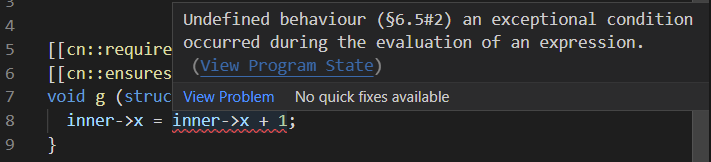
\includegraphics{figures/lsp-structs9-hover.png}
    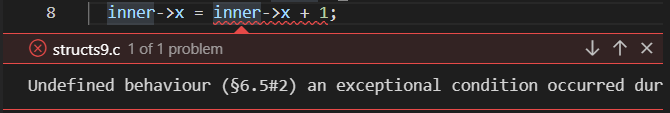
\includegraphics{figures/lsp-structs9-inline.png}
    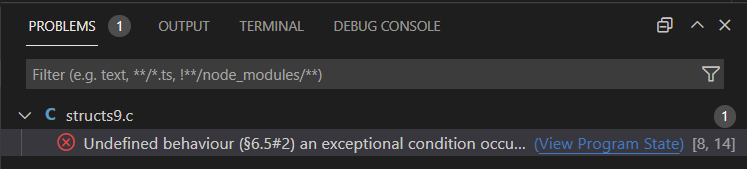
\includegraphics{figures/lsp-structs9-problems.png}
    \caption{LSP server and client I prototyped using \kl{CN}'s temperamental
    JSON output. Rather unhelpfully, it quotes the \kl{ISO} standard's jargon
    rather than explaining signed integers may not overflow.}\label{fig:lsp-extra}
\end{figure}

\paragraph{Avoid showing crashes and backtraces.} \kl{CN} does an admirable job
on controlling the effects exposed by various parts of the code by wrapping
most effectful operations in a typing monad.\sidenote{This comes with its own
trade-offs.} However, there are a few cases which result in crashes which
are predictable and avoidable if the intent is there from the beginning. The
most important reason for this is that \emph{the output from \kl{CN} can and
will be used by other tooling, to provide editor services and
GUIs}.\sidenote{For example,
\href{https://github.com/rems-project/cerberus/issues/286}{cn \-\-json
can produce non-JSON output (Cerberus\#286)} and
\href{https://github.com/rems-project/cerberus/issues/221}{Flycheck
support (Cerberus\#221)}.}\label{sn:gui-issues} At the time of writing, there are 185 uses of
\ocamlinline{failwith} and 297 uses \ocamlinline{assert} in the code
base, all of which can cause backtraces, and make it difficult for
tools to build on top of \kl{CN}. Whilst it is possible to work
around this, by calling into \kl{CN} as an OCaml library instead,
this increases the overhead of developing tooling for \kl{CN}.
These come from a couple of sources.
\begin{itemize}
    \item \textbf{Unimplemented features.} These are extremely common when
        building any large project, and so this should by no means be
        considered an exceptional condition. Instead, an error message should
        make it clear what feature is not implemented, and \emph{where in the
        source code} it rose from.
    \item \textbf{Assertion or invariant failures.} Again, whilst these signal
        bugs, bugs are common, and they need to be handled gracefully. Whilst
        backtraces may be helpful, they should not be visible by default.
\end{itemize}

\subsection{Log, do not debug}

Another regretful aspect of \kl{CN}'s development is its over-reliance on debug
output as a substitute for a user-interface and well-defined structured logs.
There are about 255 instances of debug related code in \kl{CN} today.

To be clear, I am not saying that it is necessary to invest heavily in
producing beautiful and intuitive GUIs from the start \textemdash{} that
depends on the resources available and priorities of the project.

What I am saying is that clear visibility is a trait of good software, and
unstructured debug output, whilst occasionally helpful, are rarely the first,
main or correct tool for this job. Instead, it makes much more sense to record
the sequence of actions and their effects at each step, in a reasonably
structure format so that (a) its output format can be wholly separated from the
recording and (b) processing the output can be wholly separated from both.

Structured logging is \emph{especially} useful in the presence of monadic OCaml
code, which removes all useful information from any backtraces, and inverted
control flow with explicit continuations, and manipulating state and contexts.
Whilst there is some ad hoc logging for recording the memory actions, used
for the HTML output, a disciplined logging scheme would facilitate the
following.
\begin{itemize}
    \item Profiling the solver (\cref{subsec:profile}).
    \item Validating resource inference (\cref{sec:better-foundations}).
    \item Experimenting with the user-interface.
\end{itemize}

The last one in particular has been the subject of multiple issues related to
GUIs (see note~\ref{sn:gui-issues}). It was also one of the blockers for
further progress on an LSP\sidenote{Editor-agnostic language-server protocol.}
server\sidenote{\url{https://github.com/rems-project/cn-lsp-server}} and
client\sidenote{\url{https://github.com/rems-project/cn-lsp-client}} I
prototyped (\cref{fig:lsp-state,fig:lsp-extra}).

\begin{figure*}[tp]
    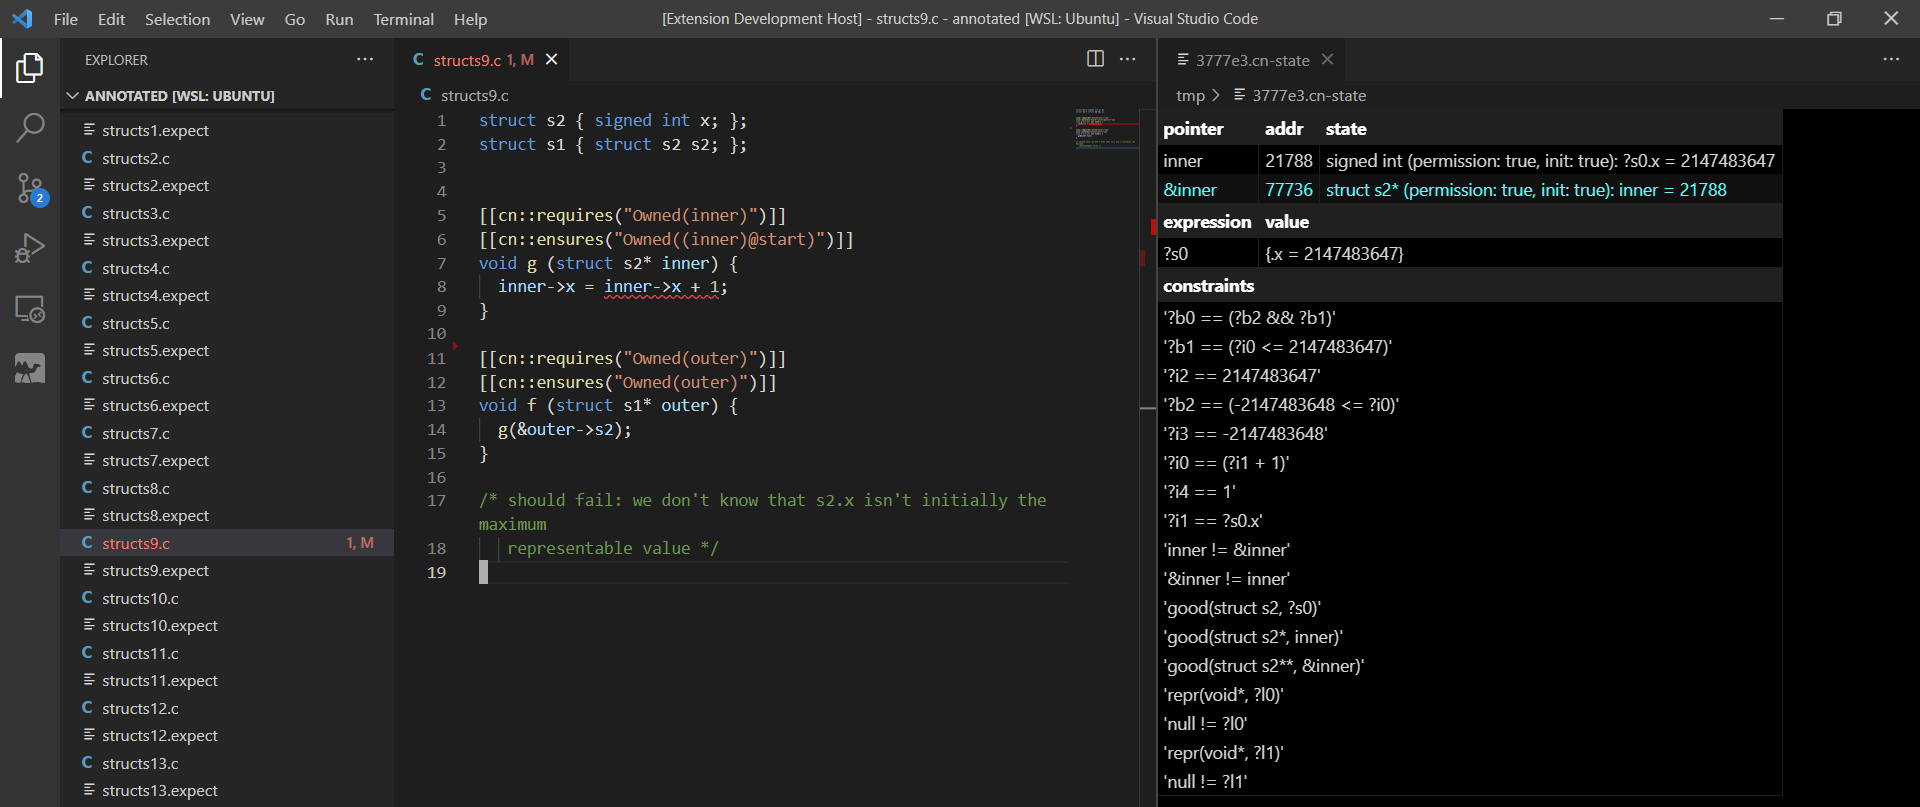
\includegraphics{figures/lsp-structs9-state.png}
    \caption{LSP server and client I prototyped using \kl{CN}'s temperamental
        JSON output. It shows the counter-example for why signed integer
        addition may cause UB.}\label{fig:lsp-state}
\end{figure*}

\subsection{Miscellaneous}

There are a myriad of other small but useful practices which have or would have
been useful regarding \kl{CN}'s development.
\begin{itemize}
    \item Gate substantial changes to \kl{CN} underneath a flag. Whilst this
        does risk making the code more complex, and accruing unused flags and
        options, the cost of breaking updates is too high, which I discussed in
        depth in \nameref{subsec:handling-large-changes}.
    \item Use version control \emph{well}. Thankfully, using version control
        these days is convenient and common, though there is an art to
        using it well.
        \begin{itemize}
            \item Break up large features into small commits. This makes them
                easier to test, review and merge piecemeal.
            \item Rebase at least daily. This simplifies the commit history and
                avoids error-prone and time-consuming merges later on.
            \item Write informative commit messages. Commit messages are just
                as much documentation as any other part of the code. A good
                message summarises the change and \emph{explains why}
                certain decision were made.
            \item If working on an online platform, work on forks, rather than
                branches. This prevents clutter on the primary repository.
        \end{itemize}
    \item Automate and enforce a continuous-integration (CI) pipeline. The
        regression testing and profiling should be there to \emph{decrease}
        developer load, rather than increase  it.
    \item Automate and enforce code formatting. Whilst no code-formatter will
        please everyone, the easiest to read (and diff) code is consistent
        code. This saves a remarkable amount of time and effort.\sidenote{Git
            has a feature to ignore certain commits when using its blame
            features, which has minimised the impact on formatting all of the
        \kl{CN} code.}
\end{itemize}

\section{Get source locations right}

Source location information is the fundamental building block of a useful error
message, without which an error is close to useless. Unfortunately, early
versions of \kl{CN} did not give this crucial data its due leading to an
incredibly poor user experience. This is all the more disappointing because
within the OCaml ecosystem, the \kl{Menhir} parser generator makes getting this
sort of thing right a lot easier than one might initially
expect~\sidecite{pottier2016reachability}.

\subsection{Keep lexer and parser simple}

Initially, support for \kl{CN}
annotations in comments was implemented with reference to lots of global
mutable state.\sidenote{A feature of ocamllex that seems to be
under-appreciated is that each rule is an OCaml function and can be passed
arbitrary parameters, thus avoid the need to use global mutable state.}
This prevented code re-use, complicated the code and introduced subtle
location bugs because of accidentally re-using shared mutable token
buffers. I simplified the lexer and parser to avoid this, and in the
process improved and unified the error-reporting for parsing C and
\kl{CN}.\sidenote{\href{https://github.com/rems-project/cerberus/pull/252}{Cerberus\#252}.}

\subsection{Investigate strange source locations}

Strange source locations are
bugs which deserve to be investigated, or at the very least, have their
triggers documented. One such
issue\sidenote{\href{https://github.com/rems-project/cerberus/issues/382}{Cerberus\#382}.}
uncovered a subtle interaction between the `lexer hack' used to parse
C11~\sidecite{jourdan2017simple}, and a token buffer feature offered by
\kl{Menhir} for more helpful error messages. Again, the issue was mutable state
which was accidentally shared across what should be separate, fresh instances
of the lexer. The solution was to stage the creation of the lexer and its
internal state, and make this explicit in its
API.\sidenote{\href{https://github.com/rems-project/cerberus/commit/c970a43b7126560b229fb55c32ce22bfbc5d23f2}{Cerberus
c970a43b}.}

\subsection{Actually use source locations once you have them}

Once source locations are accurately recorded by the front-end, then it is
important to use them in later stages. Initially, \kl{CN}'s core term type,
used for representing SMT terms, did not support source location information.
This made for a very poor and frustrating user experience in common cases, such
as ill-formed terms, or failing constraints in a specification or a predicate.

Because the type representing this term was large, and used in many places,
this made adding the location information after the fact much more tedious and
painful, and adding new code only exacerbates this further. Eventually, I spent
about one month fixing this
problem.\sidenote{\href{https://github.com/rems-project/cerberus/pull/225}{Cerberus\#225}.}
Whilst in some cases, threading source location through was obvious,
in many cases it is not. The question then arises: is it better to have all
terms have source location information, even if some of it is approximate,
or to have missing location information, but be confident about the ones
which are not missing?

Though the user-experience of the latter seems superficially worse than the
former, \emph{a bad source location is worse than no source location}, for both
the user, and the developer who has to debug it later. Hence, missing source
location information is preferable, \textbf{so long as it documents where in
the implementation code} the missing location comes from. Here is an example,
were a resource request has failed. Below is an error message which says that
ownership of a local is not available at function exit. This means that either
some predicate is not being unfolded enough, or that a function claimed
ownership without returning it. Ideally, the error would point to where this
local was declared, where it disappeared, and the definition of that field of
in that struct. In the absence of all that information, it is safer to (a) not
attempt to display any location at all or (b) if a dummy one must be provided,
point to where in the implementation this dummy location originates.

\begin{minted}[fontsize=\footnotesize,linenos,breaklines]{text}
tests/cn/reverse.error.c:124:3: error: Missing resource for de-allocating
  return 0;
  ^~~~~~~~~
Resource needed: W<struct node>(&n3)
  which requires: W<signed int>(&&n3->head)
      other location (File "backend/cn/lib/resourceInference.ml", line 220, characters 31-38)  (arg head)
State file: file:///tmp/state__reverse.error.c__main.html
\end{minted}

\subsection{Write parser error messages if feasible}

Initially, a parse error in \kl{CN} would simply signal `unexpected token' and
exit with no other information, except a ballpark source location which was
sometimes right. This was less than helpful for a number of reasons, most
notably not telling the user what token \emph{was} expected. It is possible to
\emph{generate} very inelegant, but informative parse error messages based on
the error message format output by
\kl{Menhir}.\sidenote{\url{https://gallium.inria.fr/~fpottier/menhir/manual.html\#sec\%3Amessages\%3Aformat}}

I shall now explain how I did
this.\sidenote{\href{https://github.com/rems-project/cerberus/commit/127758764cd6efdabaaaddb60eabf40575864117}{Cerberus
12775876}.} The first line shows the sentence used to get to the error state.
This is useful for \kl{Menhir}, but is not considered to be a good source of
information for writing an error message. This is because the information in
the comments shows the production which is being parsed, and at which point in
it the error occurs. More than half of error states (629) have exactly one
production, and in this case, I generate an error message as shown at the
bottom of the excerpt.

\begin{minted}[fontsize=\footnotesize,linenos,breaklines]{py}
cn_statements: ASSERT WHILE
##
## Ends in an error in state: 1585.
##
## cn_statement -> ASSERT . LPAREN assert_expr RPAREN SEMICOLON [ .. ]
##
## The known suffix of the stack is as follows:
## ASSERT
##

parsing "cn_statement": seen "ASSERT", expecting "LPAREN assert_expr RPAREN SEMICOLON"
\end{minted}

Of course, it is better to fill these and the remainder (593) manually, as I
demonstrated for one
case.\sidenote{\href{https://github.com/rems-project/cerberus/issues/245}{Cerberus\#245}.}
Details of how best to do so are in the \kl{Menhir} manual, along with
examples and links to how \kl{CompCert} uses it for its C parser (proof that
the approach can be scaled). For the cases I did not auto-generate, I
output an message which says that an error message is missing for the state
(identified by a number), and that it can be added in the stated file. In any
case, I set up \kl{Menhir} to show exactly where and between which tokens
parsing failed, which is often enough for experienced users to fix the syntax.
\kl{Menhir} also provides functionality to check and merge its auto-generated
error messages with existing ones, so that the latter can be preserved despite
changes to the grammar.

\subsection{Consider a custom pre-processor}

The bane of any academic C tooling seems to be the preprocessor. Whilst it
faithfully preserves line numbers, and this tends to be good enough, it does
not preserve column information, which in most cases, leads to inaccurate error
messages on any code which is inside, or after a macro expansion.\sidenote{The
macro call and expansion may have the same length if one is lucky.}

We are caught between two unappealing choices: either present the error message
in terms of the preprocessed code, thus retaining accuracy but sacrificing
relevancy, or present the error message (with the wrong location) in terms of
the original code, retaining relevancy but not accuracy. \kl{CN} currently does
the latter, and given the fact that macros do often represent constants, or
function-like abstractions~(\cref{subesc:takeaway-features}), we would also
like to have them supported in \kl{CN} as well.

There are no easy solutions to this,\sidenote{Even CompCert just calls a
user-specified preprocessor.} but it appears to be a solvable problem. For
example, there maybe ways to coax GCC or Clang to output debug tokens whilst
preprocessing a file, which could be input to a custom lexer which takes the
tokens \emph{and the source location information} output and connects it to the
\kl{Cerberus} front-end. Or, one could write a Clang plugin, or use the Boost
pre-processing library Wave to attempt a similar trick, with more control over
the resulting format. In both cases, it looks like it should be possible to
preserve comments too, but this will not allow running the preprocessor
\emph{inside} \kl{CN} annotations.

It may however, be feasible to implement a custom C preprocessor. What makes
this feasible is the existence of a relatively straightforward pseudo-code
algorithm by Dave Prosser, \emph{which formed the basis of the prose
    specification of macro expansion in the C89/ANSI C
standard}~\sidecite{prosser1986complete}. This algorithm is annotated and
explained~\sidecite{spinellis2008complete} by the author of the CScout
refactoring browser for C~\sidecite{spinellis2010cscout}, Diomodis
Spinellis, who was struggling to implement a C preprocessor correctly for about
five years, before finding a reference to an algorithm by Dave Prosser.
Spinellis could not find the algorithm, so he emailed Prosser who
obliged.\sidenote{\url{https://www.spinellis.gr/blog/20060626/}}

Not only is there an algorithm, Spinellis' implementation is available
online\sidenote{\url{https://github.com/dspinellis/cscout/blob/master/src/macro.cpp}}
along with a suite of test
cases\sidenote{\url{https://github.com/dspinellis/cscout/tree/master/src/test/cpp}}
and expected
outputs.\sidenote{\url{https://github.com/dspinellis/cscout/tree/master/src/test/out}}
There is even expertise within the programming language research community on
the algorithm, since it was recently discussed as being closely related to the
strategy for checking termination for expanding type definitions in type
expressions in OCaml~\sidecite{chataing2024unboxed}. This is not to say that it
will be easy, but at this stage such an effort seems more likely to succeed
than the tree-carver was when I embarked on implementing it.

\section{Process counter-examples smartly}\label{sec:counter-ex}

Whilst counter-examples have the potential to be very useful for explaining
abstract proof errors, their use in \kl{CN} is far from that currently.
The criteria represent real usability issues we have encountered with
counter-examples, but it is not clear to me how achievable they are.
In the idea world, we would aim for `dynamic witnesses for static errors',
as described in~\sidetextcite{seidel2016dynamic}.
\begin{itemize}
    \item \textbf{Multiple counter-examples may need to be shown.}
        If there is more than one predicate in the context with a matching
        name, but unequal arguments, then the counter-example will be of
        the most recent failure. A user is unable to understand why a resource
        did not match one of the ones in the middle based on the presented
        values.
    \item \textbf{Unconstrained/irrelevant variables should be excluded from the
        counter-example.} A given error will have many variables irrelevant
        to the whole program state, but the counter-example will give
        assignments to all of them, without saying which ones are directly
        relevant. This makes the user work harder to filter out irrelevant details.
    \item \textbf{Counter-examples should be consistent.} The counter-examples
        need not be consistent with respect to the irrelevant variables, and this
        can be confusing to the user too.
    \item \textbf{Counter-example variables should be easy to relate to
        program variables.} Currently, counter-example variables are presented
        in terms of symbolic variables \emph{from the precondition} of the
        function rather the values of the program variables at the point
        of failure. This means the user has to trace and work out values
        at that point for themselves.
    \item \textbf{Counter-example variables should be easy to relate to
        \emph{prior source steps}.} In general, the counter-examples represents
        the failure at the \emph{latest} step, and what users would like would
        be to see how a counter-example would evolve \emph{at every step
        leading to that}.
    \item \textbf{Counter-example values should be small.} Large numbers in
        counter-examples are difficult to comprehend. Ideally counter-examples
        would be rephrased in terms of smaller numbers which are easy to read
        and track mentally.
\end{itemize}

